\chapter{Alps Alpine Infrastructure Requirements Checklist}
\label{app:checklist}

\begin{figure}[H]
  \centering
  \rotatebox{90}{%
    \begin{minipage}{15.2cm}
      \centering
      \includegraphics[width=\linewidth, height=13.4cm, keepaspectratio]%
                      {Alps Alpine Cloud Infrastructure sketch.drawio.png}
      \small
      \caption{Alps Alpine Cloud Infrastructure --- Local Product Department:
               services in use, under investigation, or anticipated, arranged in
               six stages from foundation to user interface
               \cite{AlpsAlpine_Checklist}.}
      \label{fig:alps-infrastructure}
    \end{minipage}}
\end{figure}

\chapter{The CloudSov Evaluation Environment}
\label{app:cloudsov}

\section*{Running CloudSov locally}

The application runs locally and needs no cloud account, paid subscription, API
key or environment variable. It requires Python~3.10 or later, Node.js~18 or
later, and \texttt{npm}.

\begin{enumerate}
  \item Clone the repository:\\
        \texttt{git clone https://github.com/aaeu-ihono/cloudsov-tool.git}
  \item Start the backend:\\
        \texttt{cd backend \&\& pip install -r requirements.txt \&\& uvicorn main:app --reload}
  \item Start the frontend:\\
        \texttt{cd frontend \&\& npm install \&\& npm run dev}
  \item Open a browser at \texttt{http://localhost:5173}
\end{enumerate}

All provider data ships with the repository, so the assessment can be reproduced
from a clean checkout with no further setup.

\section*{What the interface shows}

The application presents one module per study, reached from the navigation bar:
sovereignty scoring, readiness assessment, financial viability and technical
benchmarking. 

\begin{figure}[p]
  \centering
  \fbox{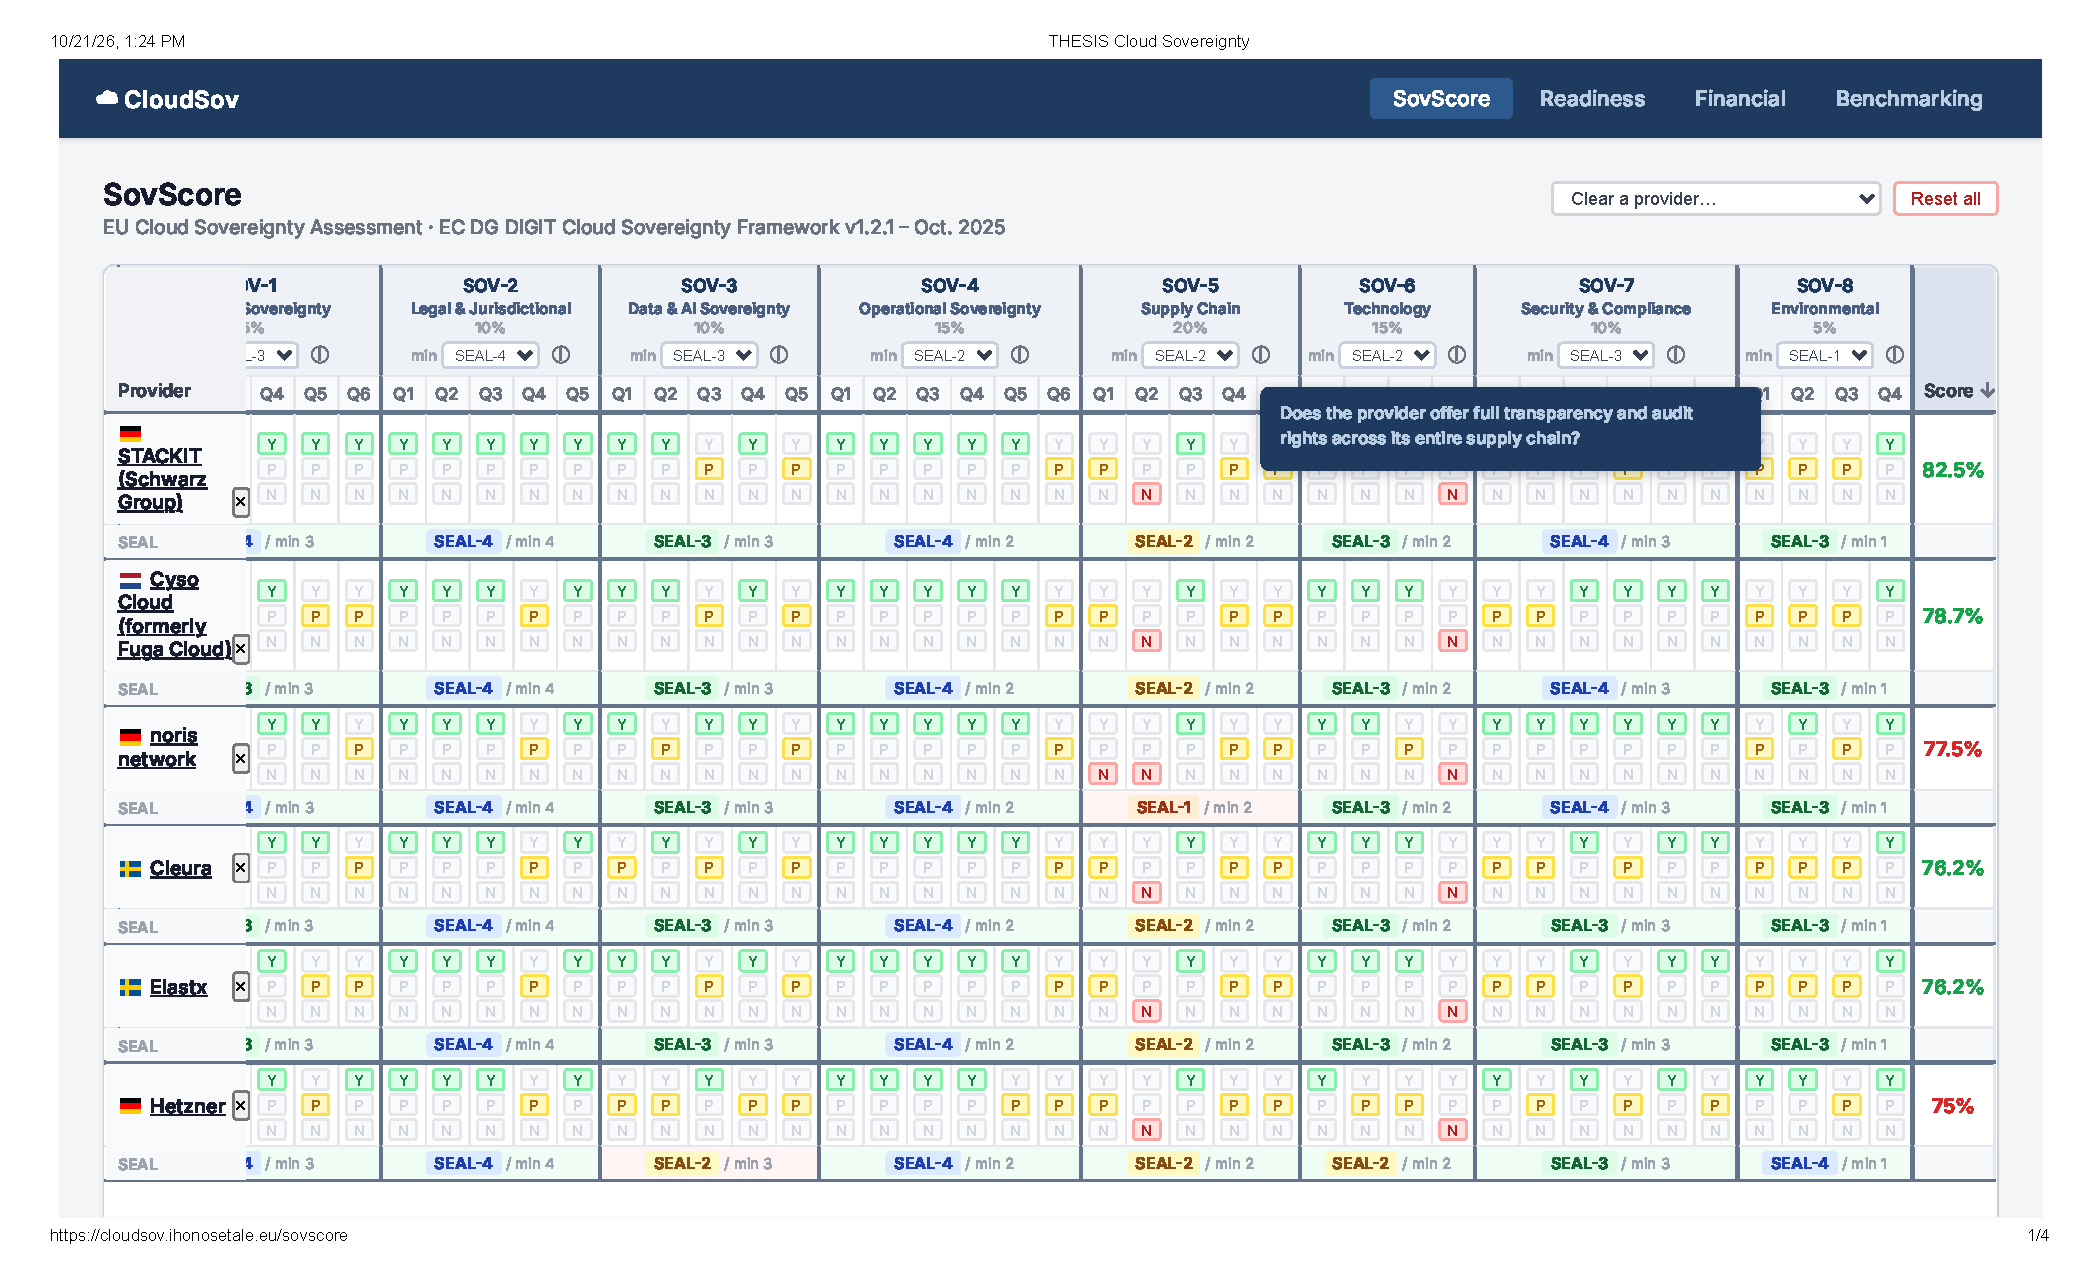
\includegraphics[page=1, width=0.97\textwidth]{print-sovscore.pdf}}

  \vspace{0.8em}
  \fbox{\includegraphics[page=2, width=0.97\textwidth]{print-sovscore.pdf}}
  \caption{The sovereignty scoring module. Each provider is a row of recorded
           verdicts, with the seal reached and the weighted score on the right.}
  \label{fig:tool-sovscore}
\end{figure}

\begin{figure}[p]
  \centering
  \fbox{\includegraphics[page=3, width=0.97\textwidth]{print-sovscore.pdf}}

  \vspace{0.4em}
  {\small The sovereignty scoring module, continued.}

  \vspace{1.2em}
  \fbox{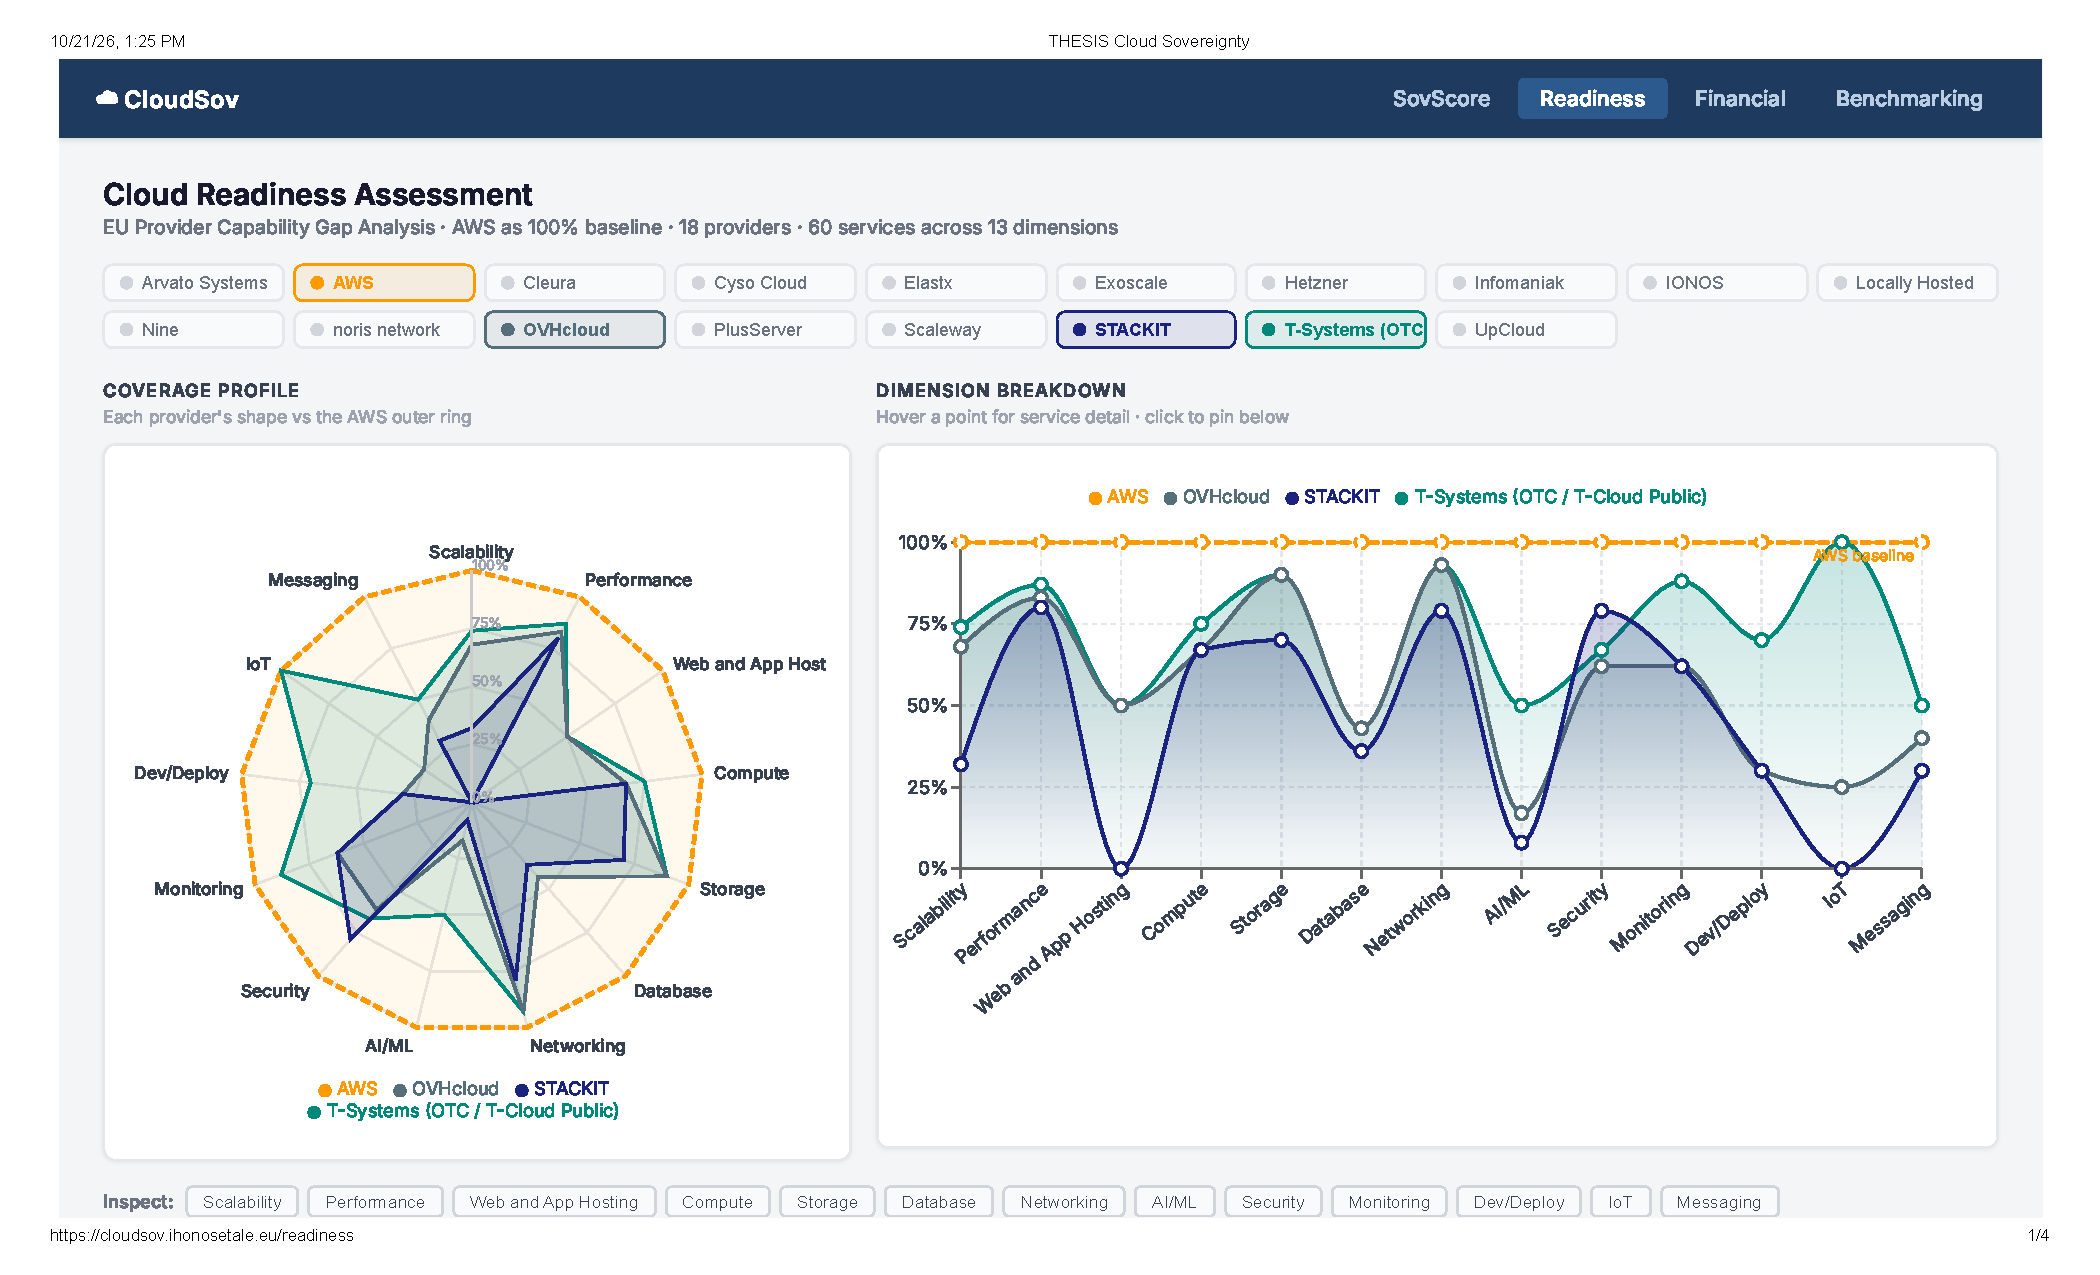
\includegraphics[page=1, width=0.97\textwidth]{print-readiness.pdf}}
  \caption{The readiness assessment module. Providers are drawn against
           \acs{AWS} by service area, with their coverage ranked beneath.}
  \label{fig:tool-readiness}
\end{figure}

\begin{figure}[p]
  \centering
  \fbox{\includegraphics[page=2, width=0.97\textwidth]{print-readiness.pdf}}

  \vspace{0.8em}
  \fbox{\includegraphics[page=3, width=0.97\textwidth]{print-readiness.pdf}}

  \vspace{0.4em}
  {\small The readiness assessment module, continued.}
\end{figure}

\begin{figure}[p]
  \centering
  \fbox{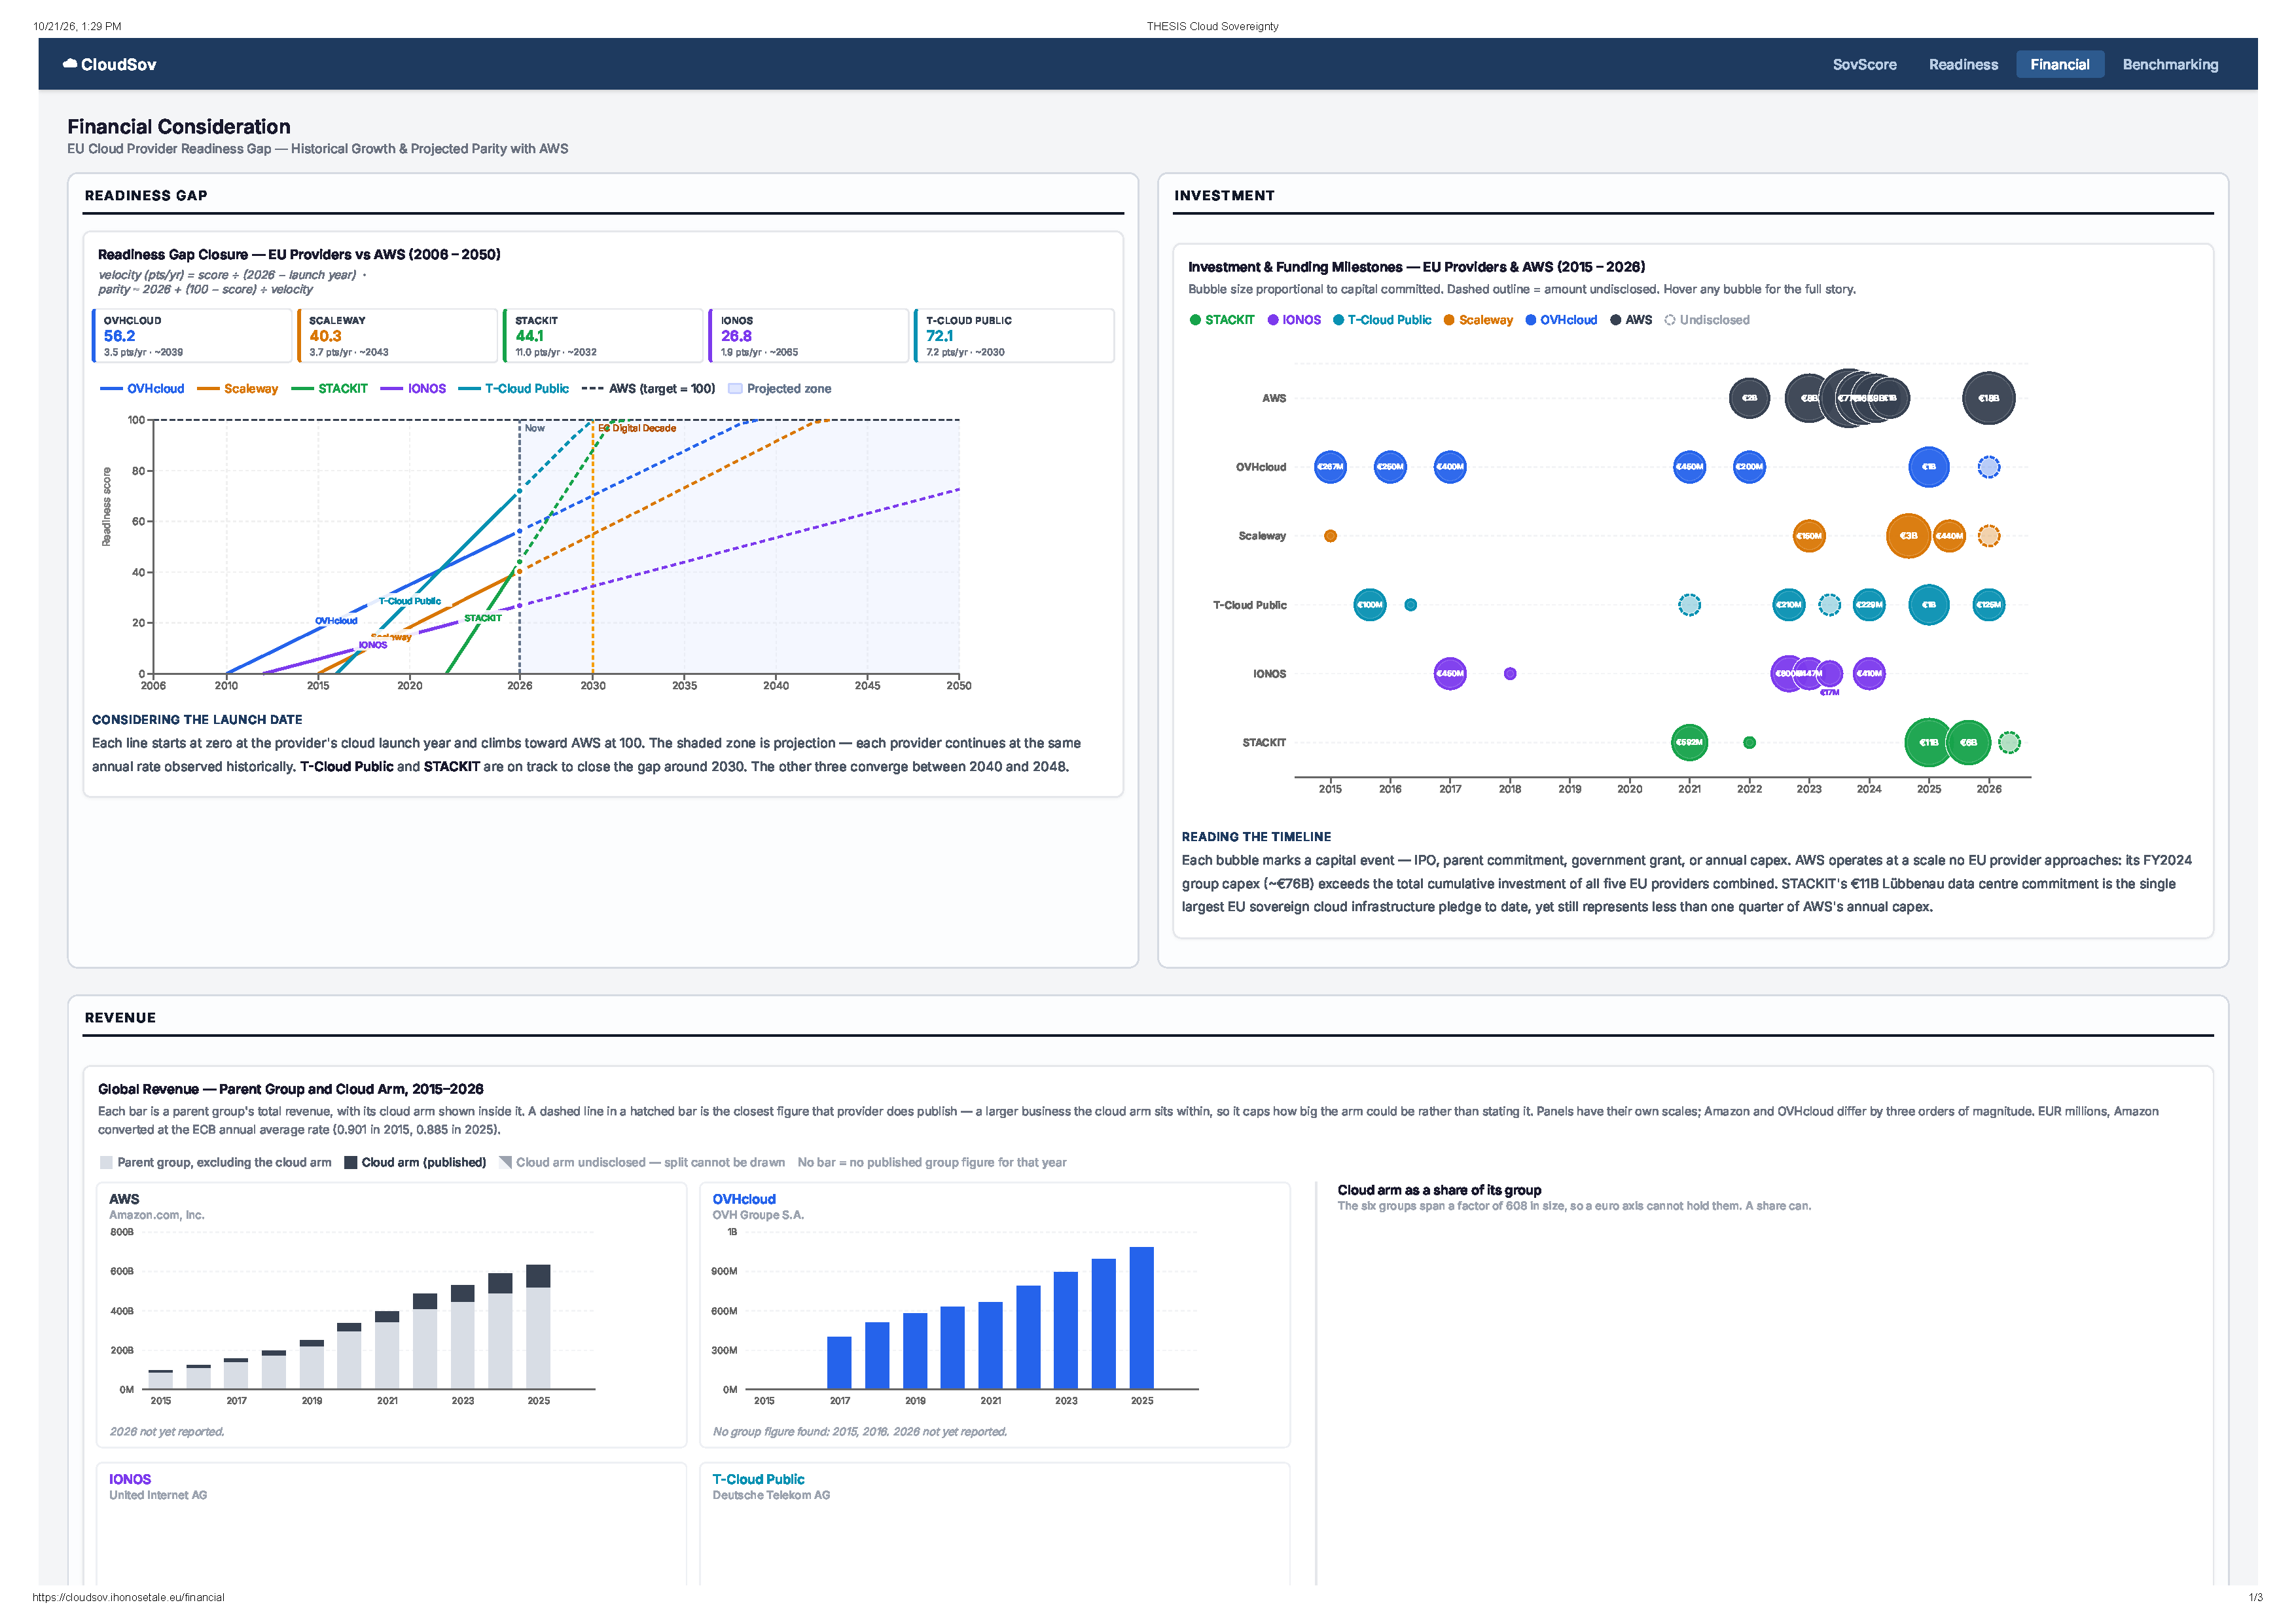
\includegraphics[page=1, width=0.97\textwidth]{print-financials.pdf}}

  \vspace{0.8em}
  \fbox{\includegraphics[page=2, width=0.97\textwidth]{print-financials.pdf}}
  \caption{The financial module. Readiness growth over time, investment
           milestones, revenue and the share of revenue earned in Europe.}
  \label{fig:tool-financial}
\end{figure}

\begin{figure}[p]
  \centering
  \fbox{\includegraphics[page=3, width=0.97\textwidth]{print-financials.pdf}}

  \vspace{0.4em}
  {\small The financial module, continued.}
\end{figure}

\begin{figure}[p]
  \centering
  \fbox{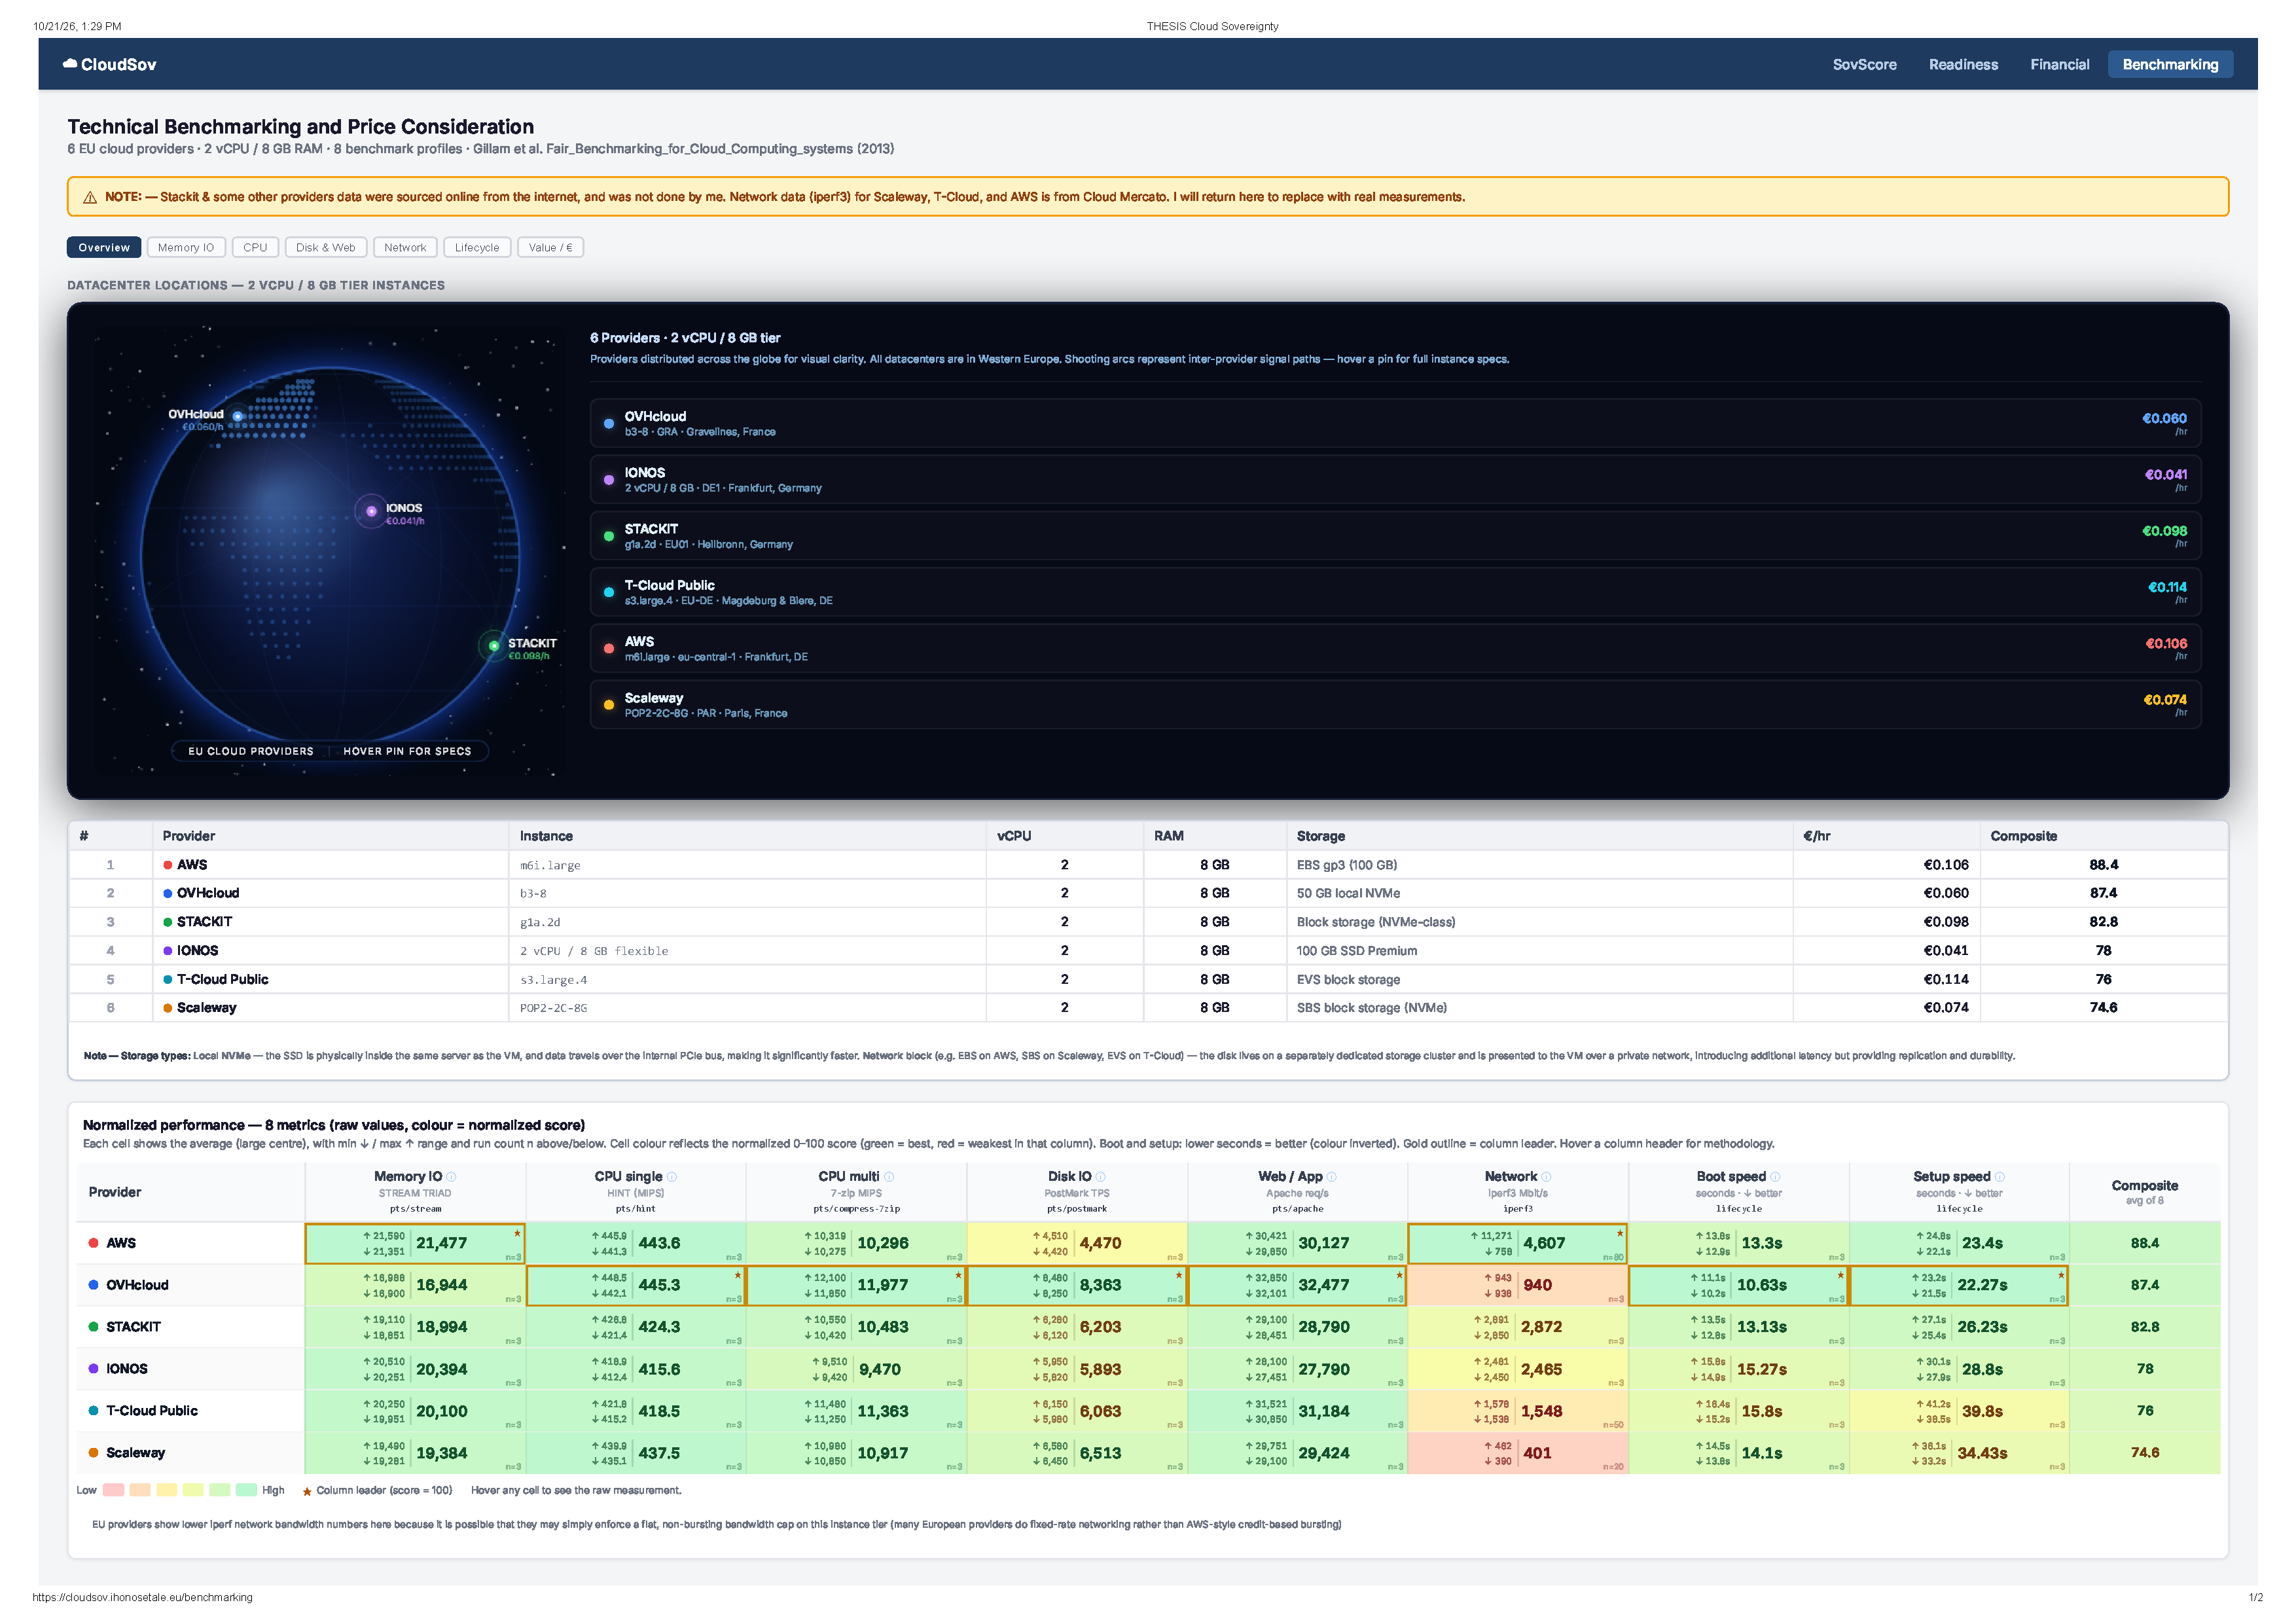
\includegraphics[page=1, width=0.97\textwidth]{print-benchmark.pdf}}

  \vspace{0.8em}
  \fbox{\includegraphics[page=2, width=0.97\textwidth]{print-benchmark.pdf}}
  \caption{The technical benchmarking module. Instance prices, the measured
           results for each test and the combined performance score.}
  \label{fig:tool-benchmark}
\end{figure}

\chapter{Sovereignty Assessment Evidence}
\label{app:sov-evidence}

\Cref{tab:sov-verdicts} gives the answer each provider received on each of the
forty-one sovereignty questions of \cref{sec:method-study1}: yes, partly or no.
Providers are listed in the order of their overall score in \cref{fig:sov-ranking}.
For every answer, the reasoning behind it and the link to the published document it
rests on are stored with the data in the CloudSov repository, in one file per
provider in the folder \texttt{sovscore} (\cref{app:cloudsov}).

\begin{table}[p]
  \centering
  \caption{Answers to the forty-one sovereignty questions, by provider.}
  \label{tab:sov-verdicts}
  \tiny
  \setlength{\tabcolsep}{1.6pt}
  \renewcommand{\arraystretch}{1.05}
  \begin{tabular}{@{}l l *{18}{c}@{}}
    \toprule
    & \textbf{Question} & \rotatebox{90}{STACKIT} & \rotatebox{90}{Cyso Cloud} & \rotatebox{90}{noris network} & \rotatebox{90}{Cleura} & \rotatebox{90}{Elastx} & \rotatebox{90}{Hetzner} & \rotatebox{90}{Scaleway} & \rotatebox{90}{plusserver} & \rotatebox{90}{Exoscale} & \rotatebox{90}{T-Cloud Public} & \rotatebox{90}{Infomaniak} & \rotatebox{90}{UpCloud} & \rotatebox{90}{OVHcloud} & \rotatebox{90}{Nine} & \rotatebox{90}{IONOS} & \rotatebox{90}{Locally hosted} & \rotatebox{90}{Arvato Systems} & \rotatebox{90}{Open Telekom Cloud} \\
    \midrule
SOV-1 Q1 & Decisive authority within the EU & \cellcolor{green!22}Y & \cellcolor{green!22}Y & \cellcolor{green!22}Y & \cellcolor{orange!25}P & \cellcolor{green!22}Y & \cellcolor{green!22}Y & \cellcolor{green!22}Y & \cellcolor{orange!25}P & \cellcolor{red!25}N & \cellcolor{green!22}Y & \cellcolor{orange!25}P & \cellcolor{green!22}Y & \cellcolor{green!22}Y & \cellcolor{orange!25}P & \cellcolor{orange!25}P & \cellcolor{green!22}Y & \cellcolor{green!22}Y & \cellcolor{orange!25}P \\
SOV-1 Q2 & Protected against non-EU takeover & \cellcolor{green!22}Y & \cellcolor{orange!25}P & \cellcolor{green!22}Y & \cellcolor{orange!25}P & \cellcolor{orange!25}P & \cellcolor{green!22}Y & \cellcolor{green!22}Y & \cellcolor{orange!25}P & \cellcolor{orange!25}P & \cellcolor{orange!25}P & \cellcolor{green!22}Y & \cellcolor{orange!25}P & \cellcolor{orange!25}P & \cellcolor{orange!25}P & \cellcolor{red!25}N & \cellcolor{green!22}Y & \cellcolor{orange!25}P & \cellcolor{orange!25}P \\
SOV-1 Q3 & Financed from within the EU & \cellcolor{green!22}Y & \cellcolor{green!22}Y & \cellcolor{green!22}Y & \cellcolor{orange!25}P & \cellcolor{green!22}Y & \cellcolor{green!22}Y & \cellcolor{orange!25}P & \cellcolor{orange!25}P & \cellcolor{orange!25}P & \cellcolor{green!22}Y & \cellcolor{green!22}Y & \cellcolor{green!22}Y & \cellcolor{orange!25}P & \cellcolor{green!22}Y & \cellcolor{orange!25}P & \cellcolor{orange!25}P & \cellcolor{orange!25}P & \cellcolor{orange!25}P \\
SOV-1 Q4 & Invests and employs in the EU & \cellcolor{green!22}Y & \cellcolor{green!22}Y & \cellcolor{green!22}Y & \cellcolor{green!22}Y & \cellcolor{green!22}Y & \cellcolor{green!22}Y & \cellcolor{green!22}Y & \cellcolor{green!22}Y & \cellcolor{green!22}Y & \cellcolor{green!22}Y & \cellcolor{orange!25}P & \cellcolor{green!22}Y & \cellcolor{green!22}Y & \cellcolor{orange!25}P & \cellcolor{green!22}Y & \cellcolor{orange!25}P & \cellcolor{green!22}Y & \cellcolor{green!22}Y \\
SOV-1 Q5 & Active in EU sovereignty work & \cellcolor{green!22}Y & \cellcolor{orange!25}P & \cellcolor{green!22}Y & \cellcolor{green!22}Y & \cellcolor{orange!25}P & \cellcolor{orange!25}P & \cellcolor{green!22}Y & \cellcolor{green!22}Y & \cellcolor{green!22}Y & \cellcolor{green!22}Y & \cellcolor{orange!25}P & \cellcolor{orange!25}P & \cellcolor{green!22}Y & \cellcolor{orange!25}P & \cellcolor{green!22}Y & \cellcolor{red!25}N & \cellcolor{green!22}Y & \cellcolor{orange!25}P \\
SOV-1 Q6 & Survives withdrawal of vendor support & \cellcolor{green!22}Y & \cellcolor{orange!25}P & \cellcolor{orange!25}P & \cellcolor{orange!25}P & \cellcolor{orange!25}P & \cellcolor{green!22}Y & \cellcolor{green!22}Y & \cellcolor{orange!25}P & \cellcolor{orange!25}P & \cellcolor{orange!25}P & \cellcolor{green!22}Y & \cellcolor{orange!25}P & \cellcolor{orange!25}P & \cellcolor{orange!25}P & \cellcolor{orange!25}P & \cellcolor{orange!25}P & \cellcolor{orange!25}P & \cellcolor{red!25}N \\
\midrule
SOV-2 Q1 & Governed only by member-state law & \cellcolor{green!22}Y & \cellcolor{green!22}Y & \cellcolor{green!22}Y & \cellcolor{green!22}Y & \cellcolor{green!22}Y & \cellcolor{green!22}Y & \cellcolor{green!22}Y & \cellcolor{green!22}Y & \cellcolor{orange!25}P & \cellcolor{green!22}Y & \cellcolor{red!25}N & \cellcolor{green!22}Y & \cellcolor{orange!25}P & \cellcolor{red!25}N & \cellcolor{orange!25}P & \cellcolor{green!22}Y & \cellcolor{green!22}Y & \cellcolor{green!22}Y \\
SOV-2 Q2 & Free of laws with reach from abroad & \cellcolor{green!22}Y & \cellcolor{green!22}Y & \cellcolor{green!22}Y & \cellcolor{green!22}Y & \cellcolor{green!22}Y & \cellcolor{green!22}Y & \cellcolor{green!22}Y & \cellcolor{green!22}Y & \cellcolor{green!22}Y & \cellcolor{orange!25}P & \cellcolor{green!22}Y & \cellcolor{orange!25}P & \cellcolor{orange!25}P & \cellcolor{green!22}Y & \cellcolor{orange!25}P & \cellcolor{green!22}Y & \cellcolor{orange!25}P & \cellcolor{orange!25}P \\
SOV-2 Q3 & No channel for forced access & \cellcolor{green!22}Y & \cellcolor{green!22}Y & \cellcolor{green!22}Y & \cellcolor{green!22}Y & \cellcolor{green!22}Y & \cellcolor{green!22}Y & \cellcolor{green!22}Y & \cellcolor{green!22}Y & \cellcolor{green!22}Y & \cellcolor{orange!25}P & \cellcolor{green!22}Y & \cellcolor{green!22}Y & \cellcolor{red!25}N & \cellcolor{green!22}Y & \cellcolor{orange!25}P & \cellcolor{green!22}Y & \cellcolor{orange!25}P & \cellcolor{red!25}N \\
SOV-2 Q4 & Free of export-control rules & \cellcolor{green!22}Y & \cellcolor{orange!25}P & \cellcolor{orange!25}P & \cellcolor{orange!25}P & \cellcolor{orange!25}P & \cellcolor{orange!25}P & \cellcolor{orange!25}P & \cellcolor{orange!25}P & \cellcolor{orange!25}P & \cellcolor{orange!25}P & \cellcolor{orange!25}P & \cellcolor{orange!25}P & \cellcolor{orange!25}P & \cellcolor{orange!25}P & \cellcolor{orange!25}P & \cellcolor{green!22}Y & \cellcolor{orange!25}P & \cellcolor{orange!25}P \\
SOV-2 Q5 & Intellectual property EU-owned & \cellcolor{green!22}Y & \cellcolor{green!22}Y & \cellcolor{green!22}Y & \cellcolor{green!22}Y & \cellcolor{green!22}Y & \cellcolor{green!22}Y & \cellcolor{orange!25}P & \cellcolor{green!22}Y & \cellcolor{orange!25}P & \cellcolor{red!25}N & \cellcolor{orange!25}P & \cellcolor{orange!25}P & \cellcolor{orange!25}P & \cellcolor{orange!25}P & \cellcolor{orange!25}P & \cellcolor{orange!25}P & \cellcolor{orange!25}P & \cellcolor{red!25}N \\
\midrule
SOV-3 Q1 & Customer holds the encryption keys & \cellcolor{green!22}Y & \cellcolor{green!22}Y & \cellcolor{green!22}Y & \cellcolor{orange!25}P & \cellcolor{green!22}Y & \cellcolor{orange!25}P & \cellcolor{green!22}Y & \cellcolor{orange!25}P & \cellcolor{green!22}Y & \cellcolor{green!22}Y & \cellcolor{orange!25}P & \cellcolor{orange!25}P & \cellcolor{orange!25}P & \cellcolor{orange!25}P & \cellcolor{orange!25}P & \cellcolor{green!22}Y & \cellcolor{orange!25}P & \cellcolor{green!22}Y \\
SOV-3 Q2 & Access to data and AI auditable & \cellcolor{green!22}Y & \cellcolor{green!22}Y & \cellcolor{orange!25}P & \cellcolor{green!22}Y & \cellcolor{green!22}Y & \cellcolor{orange!25}P & \cellcolor{green!22}Y & \cellcolor{green!22}Y & \cellcolor{orange!25}P & \cellcolor{orange!25}P & \cellcolor{orange!25}P & \cellcolor{orange!25}P & \cellcolor{orange!25}P & \cellcolor{orange!25}P & \cellcolor{green!22}Y & \cellcolor{orange!25}P & \cellcolor{orange!25}P & \cellcolor{orange!25}P \\
SOV-3 Q3 & Deletion verifiable and final & \cellcolor{orange!25}P & \cellcolor{orange!25}P & \cellcolor{green!22}Y & \cellcolor{orange!25}P & \cellcolor{orange!25}P & \cellcolor{green!22}Y & \cellcolor{green!22}Y & \cellcolor{orange!25}P & \cellcolor{orange!25}P & \cellcolor{orange!25}P & \cellcolor{orange!25}P & \cellcolor{orange!25}P & \cellcolor{green!22}Y & \cellcolor{orange!25}P & \cellcolor{orange!25}P & \cellcolor{orange!25}P & \cellcolor{orange!25}P & \cellcolor{orange!25}P \\
SOV-3 Q4 & Storage and processing EU-only & \cellcolor{green!22}Y & \cellcolor{green!22}Y & \cellcolor{green!22}Y & \cellcolor{green!22}Y & \cellcolor{green!22}Y & \cellcolor{orange!25}P & \cellcolor{green!22}Y & \cellcolor{green!22}Y & \cellcolor{green!22}Y & \cellcolor{green!22}Y & \cellcolor{orange!25}P & \cellcolor{orange!25}P & \cellcolor{orange!25}P & \cellcolor{orange!25}P & \cellcolor{orange!25}P & \cellcolor{green!22}Y & \cellcolor{green!22}Y & \cellcolor{green!22}Y \\
SOV-3 Q5 & AI models governed in the EU & \cellcolor{orange!25}P & \cellcolor{orange!25}P & \cellcolor{orange!25}P & \cellcolor{orange!25}P & \cellcolor{orange!25}P & \cellcolor{orange!25}P & \cellcolor{orange!25}P & \cellcolor{orange!25}P & \cellcolor{orange!25}P & \cellcolor{orange!25}P & \cellcolor{orange!25}P & \cellcolor{orange!25}P & \cellcolor{orange!25}P & \cellcolor{orange!25}P & \cellcolor{orange!25}P & \cellcolor{orange!25}P & \cellcolor{orange!25}P & \cellcolor{orange!25}P \\
\midrule
SOV-4 Q1 & Workloads movable without lock-in & \cellcolor{green!22}Y & \cellcolor{green!22}Y & \cellcolor{green!22}Y & \cellcolor{green!22}Y & \cellcolor{green!22}Y & \cellcolor{green!22}Y & \cellcolor{green!22}Y & \cellcolor{green!22}Y & \cellcolor{green!22}Y & \cellcolor{green!22}Y & \cellcolor{green!22}Y & \cellcolor{green!22}Y & \cellcolor{green!22}Y & \cellcolor{green!22}Y & \cellcolor{green!22}Y & \cellcolor{orange!25}P & \cellcolor{orange!25}P & \cellcolor{green!22}Y \\
SOV-4 Q2 & EU operators can run it alone & \cellcolor{green!22}Y & \cellcolor{green!22}Y & \cellcolor{green!22}Y & \cellcolor{green!22}Y & \cellcolor{green!22}Y & \cellcolor{green!22}Y & \cellcolor{green!22}Y & \cellcolor{orange!25}P & \cellcolor{green!22}Y & \cellcolor{orange!25}P & \cellcolor{green!22}Y & \cellcolor{green!22}Y & \cellcolor{orange!25}P & \cellcolor{green!22}Y & \cellcolor{orange!25}P & \cellcolor{orange!25}P & \cellcolor{orange!25}P & \cellcolor{red!25}N \\
SOV-4 Q3 & EU talent pool exists & \cellcolor{green!22}Y & \cellcolor{green!22}Y & \cellcolor{green!22}Y & \cellcolor{green!22}Y & \cellcolor{green!22}Y & \cellcolor{green!22}Y & \cellcolor{green!22}Y & \cellcolor{green!22}Y & \cellcolor{green!22}Y & \cellcolor{green!22}Y & \cellcolor{orange!25}P & \cellcolor{green!22}Y & \cellcolor{green!22}Y & \cellcolor{orange!25}P & \cellcolor{green!22}Y & \cellcolor{green!22}Y & \cellcolor{green!22}Y & \cellcolor{green!22}Y \\
SOV-4 Q4 & Support delivered from the EU & \cellcolor{green!22}Y & \cellcolor{green!22}Y & \cellcolor{green!22}Y & \cellcolor{green!22}Y & \cellcolor{green!22}Y & \cellcolor{green!22}Y & \cellcolor{green!22}Y & \cellcolor{green!22}Y & \cellcolor{green!22}Y & \cellcolor{green!22}Y & \cellcolor{orange!25}P & \cellcolor{orange!25}P & \cellcolor{orange!25}P & \cellcolor{orange!25}P & \cellcolor{orange!25}P & \cellcolor{orange!25}P & \cellcolor{orange!25}P & \cellcolor{orange!25}P \\
SOV-4 Q5 & Documentation and source available & \cellcolor{green!22}Y & \cellcolor{green!22}Y & \cellcolor{green!22}Y & \cellcolor{green!22}Y & \cellcolor{green!22}Y & \cellcolor{orange!25}P & \cellcolor{orange!25}P & \cellcolor{orange!25}P & \cellcolor{orange!25}P & \cellcolor{orange!25}P & \cellcolor{green!22}Y & \cellcolor{orange!25}P & \cellcolor{green!22}Y & \cellcolor{green!22}Y & \cellcolor{green!22}Y & \cellcolor{orange!25}P & \cellcolor{orange!25}P & \cellcolor{orange!25}P \\
SOV-4 Q6 & Subcontractors under EU law & \cellcolor{orange!25}P & \cellcolor{orange!25}P & \cellcolor{orange!25}P & \cellcolor{orange!25}P & \cellcolor{orange!25}P & \cellcolor{orange!25}P & \cellcolor{orange!25}P & \cellcolor{orange!25}P & \cellcolor{orange!25}P & \cellcolor{red!25}N & \cellcolor{orange!25}P & \cellcolor{green!22}Y & \cellcolor{orange!25}P & \cellcolor{orange!25}P & \cellcolor{orange!25}P & \cellcolor{red!25}N & \cellcolor{red!25}N & \cellcolor{red!25}N \\
\midrule
SOV-5 Q1 & Hardware made in trusted countries & \cellcolor{orange!25}P & \cellcolor{orange!25}P & \cellcolor{red!25}N & \cellcolor{orange!25}P & \cellcolor{orange!25}P & \cellcolor{orange!25}P & \cellcolor{orange!25}P & \cellcolor{orange!25}P & \cellcolor{orange!25}P & \cellcolor{orange!25}P & \cellcolor{orange!25}P & \cellcolor{orange!25}P & \cellcolor{green!22}Y & \cellcolor{orange!25}P & \cellcolor{orange!25}P & \cellcolor{orange!25}P & \cellcolor{orange!25}P & \cellcolor{red!25}N \\
SOV-5 Q2 & Firmware of EU origin & \cellcolor{red!25}N & \cellcolor{red!25}N & \cellcolor{red!25}N & \cellcolor{red!25}N & \cellcolor{red!25}N & \cellcolor{red!25}N & \cellcolor{red!25}N & \cellcolor{red!25}N & \cellcolor{red!25}N & \cellcolor{red!25}N & \cellcolor{red!25}N & \cellcolor{red!25}N & \cellcolor{red!25}N & \cellcolor{red!25}N & \cellcolor{red!25}N & \cellcolor{red!25}N & \cellcolor{red!25}N & \cellcolor{red!25}N \\
SOV-5 Q3 & Software built and updated in the EU & \cellcolor{green!22}Y & \cellcolor{green!22}Y & \cellcolor{green!22}Y & \cellcolor{green!22}Y & \cellcolor{green!22}Y & \cellcolor{green!22}Y & \cellcolor{orange!25}P & \cellcolor{green!22}Y & \cellcolor{green!22}Y & \cellcolor{orange!25}P & \cellcolor{orange!25}P & \cellcolor{orange!25}P & \cellcolor{orange!25}P & \cellcolor{orange!25}P & \cellcolor{orange!25}P & \cellcolor{orange!25}P & \cellcolor{orange!25}P & \cellcolor{orange!25}P \\
SOV-5 Q4 & Free of reliance on non-EU vendors & \cellcolor{orange!25}P & \cellcolor{orange!25}P & \cellcolor{orange!25}P & \cellcolor{orange!25}P & \cellcolor{orange!25}P & \cellcolor{orange!25}P & \cellcolor{orange!25}P & \cellcolor{orange!25}P & \cellcolor{orange!25}P & \cellcolor{red!25}N & \cellcolor{orange!25}P & \cellcolor{orange!25}P & \cellcolor{orange!25}P & \cellcolor{orange!25}P & \cellcolor{orange!25}P & \cellcolor{red!25}N & \cellcolor{red!25}N & \cellcolor{red!25}N \\
SOV-5 Q5 & Supply chain auditable end to end & \cellcolor{orange!25}P & \cellcolor{orange!25}P & \cellcolor{orange!25}P & \cellcolor{orange!25}P & \cellcolor{orange!25}P & \cellcolor{orange!25}P & \cellcolor{orange!25}P & \cellcolor{orange!25}P & \cellcolor{orange!25}P & \cellcolor{orange!25}P & \cellcolor{orange!25}P & \cellcolor{orange!25}P & \cellcolor{orange!25}P & \cellcolor{orange!25}P & \cellcolor{orange!25}P & \cellcolor{orange!25}P & \cellcolor{orange!25}P & \cellcolor{orange!25}P \\
\midrule
SOV-6 Q1 & Open standards and documented APIs & \cellcolor{green!22}Y & \cellcolor{green!22}Y & \cellcolor{green!22}Y & \cellcolor{green!22}Y & \cellcolor{green!22}Y & \cellcolor{green!22}Y & \cellcolor{green!22}Y & \cellcolor{green!22}Y & \cellcolor{green!22}Y & \cellcolor{green!22}Y & \cellcolor{green!22}Y & \cellcolor{green!22}Y & \cellcolor{green!22}Y & \cellcolor{green!22}Y & \cellcolor{green!22}Y & \cellcolor{orange!25}P & \cellcolor{orange!25}P & \cellcolor{green!22}Y \\
SOV-6 Q2 & Stack open-source and modifiable & \cellcolor{green!22}Y & \cellcolor{green!22}Y & \cellcolor{green!22}Y & \cellcolor{green!22}Y & \cellcolor{green!22}Y & \cellcolor{orange!25}P & \cellcolor{orange!25}P & \cellcolor{orange!25}P & \cellcolor{orange!25}P & \cellcolor{orange!25}P & \cellcolor{green!22}Y & \cellcolor{orange!25}P & \cellcolor{orange!25}P & \cellcolor{green!22}Y & \cellcolor{orange!25}P & \cellcolor{orange!25}P & \cellcolor{red!25}N & \cellcolor{orange!25}P \\
SOV-6 Q3 & Architecture and dependencies disclosed & \cellcolor{green!22}Y & \cellcolor{green!22}Y & \cellcolor{orange!25}P & \cellcolor{green!22}Y & \cellcolor{green!22}Y & \cellcolor{orange!25}P & \cellcolor{orange!25}P & \cellcolor{orange!25}P & \cellcolor{orange!25}P & \cellcolor{orange!25}P & \cellcolor{orange!25}P & \cellcolor{orange!25}P & \cellcolor{orange!25}P & \cellcolor{orange!25}P & \cellcolor{orange!25}P & \cellcolor{green!22}Y & \cellcolor{orange!25}P & \cellcolor{orange!25}P \\
SOV-6 Q4 & Free of non-EU high-performance chips & \cellcolor{red!25}N & \cellcolor{red!25}N & \cellcolor{red!25}N & \cellcolor{red!25}N & \cellcolor{red!25}N & \cellcolor{red!25}N & \cellcolor{red!25}N & \cellcolor{red!25}N & \cellcolor{red!25}N & \cellcolor{red!25}N & \cellcolor{red!25}N & \cellcolor{red!25}N & \cellcolor{red!25}N & \cellcolor{red!25}N & \cellcolor{red!25}N & \cellcolor{red!25}N & \cellcolor{red!25}N & \cellcolor{red!25}N \\
\midrule
SOV-7 Q1 & Holds recognised EU certifications & \cellcolor{green!22}Y & \cellcolor{orange!25}P & \cellcolor{green!22}Y & \cellcolor{orange!25}P & \cellcolor{orange!25}P & \cellcolor{green!22}Y & \cellcolor{orange!25}P & \cellcolor{green!22}Y & \cellcolor{green!22}Y & \cellcolor{green!22}Y & \cellcolor{orange!25}P & \cellcolor{orange!25}P & \cellcolor{orange!25}P & \cellcolor{orange!25}P & \cellcolor{orange!25}P & \cellcolor{red!25}N & \cellcolor{green!22}Y & \cellcolor{green!22}Y \\
SOV-7 Q2 & Compliant with GDPR, NIS2, DORA & \cellcolor{green!22}Y & \cellcolor{orange!25}P & \cellcolor{green!22}Y & \cellcolor{orange!25}P & \cellcolor{orange!25}P & \cellcolor{orange!25}P & \cellcolor{orange!25}P & \cellcolor{green!22}Y & \cellcolor{green!22}Y & \cellcolor{green!22}Y & \cellcolor{orange!25}P & \cellcolor{green!22}Y & \cellcolor{green!22}Y & \cellcolor{orange!25}P & \cellcolor{green!22}Y & \cellcolor{orange!25}P & \cellcolor{green!22}Y & \cellcolor{green!22}Y \\
SOV-7 Q3 & Security operations under EU law & \cellcolor{green!22}Y & \cellcolor{green!22}Y & \cellcolor{green!22}Y & \cellcolor{green!22}Y & \cellcolor{green!22}Y & \cellcolor{green!22}Y & \cellcolor{green!22}Y & \cellcolor{green!22}Y & \cellcolor{green!22}Y & \cellcolor{green!22}Y & \cellcolor{orange!25}P & \cellcolor{orange!25}P & \cellcolor{orange!25}P & \cellcolor{orange!25}P & \cellcolor{orange!25}P & \cellcolor{orange!25}P & \cellcolor{green!22}Y & \cellcolor{green!22}Y \\
SOV-7 Q4 & Customer oversight of monitoring & \cellcolor{orange!25}P & \cellcolor{green!22}Y & \cellcolor{green!22}Y & \cellcolor{orange!25}P & \cellcolor{orange!25}P & \cellcolor{orange!25}P & \cellcolor{orange!25}P & \cellcolor{green!22}Y & \cellcolor{green!22}Y & \cellcolor{orange!25}P & \cellcolor{orange!25}P & \cellcolor{orange!25}P & \cellcolor{orange!25}P & \cellcolor{green!22}Y & \cellcolor{orange!25}P & \cellcolor{green!22}Y & \cellcolor{orange!25}P & \cellcolor{green!22}Y \\
SOV-7 Q5 & EU-compliant breach reporting & \cellcolor{green!22}Y & \cellcolor{green!22}Y & \cellcolor{green!22}Y & \cellcolor{green!22}Y & \cellcolor{green!22}Y & \cellcolor{green!22}Y & \cellcolor{green!22}Y & \cellcolor{green!22}Y & \cellcolor{green!22}Y & \cellcolor{green!22}Y & \cellcolor{green!22}Y & \cellcolor{green!22}Y & \cellcolor{green!22}Y & \cellcolor{green!22}Y & \cellcolor{green!22}Y & \cellcolor{orange!25}P & \cellcolor{green!22}Y & \cellcolor{orange!25}P \\
SOV-7 Q6 & Independent audits permitted & \cellcolor{green!22}Y & \cellcolor{green!22}Y & \cellcolor{green!22}Y & \cellcolor{green!22}Y & \cellcolor{green!22}Y & \cellcolor{orange!25}P & \cellcolor{orange!25}P & \cellcolor{green!22}Y & \cellcolor{orange!25}P & \cellcolor{orange!25}P & \cellcolor{green!22}Y & \cellcolor{orange!25}P & \cellcolor{orange!25}P & \cellcolor{green!22}Y & \cellcolor{green!22}Y & \cellcolor{green!22}Y & \cellcolor{green!22}Y & \cellcolor{orange!25}P \\
\midrule
SOV-8 Q1 & Energy-efficient, with published targets & \cellcolor{orange!25}P & \cellcolor{orange!25}P & \cellcolor{orange!25}P & \cellcolor{orange!25}P & \cellcolor{orange!25}P & \cellcolor{green!22}Y & \cellcolor{orange!25}P & \cellcolor{orange!25}P & \cellcolor{orange!25}P & \cellcolor{orange!25}P & \cellcolor{green!22}Y & \cellcolor{orange!25}P & \cellcolor{orange!25}P & \cellcolor{orange!25}P & \cellcolor{orange!25}P & \cellcolor{red!25}N & \cellcolor{orange!25}P & \cellcolor{orange!25}P \\
SOV-8 Q2 & Circular practices for hardware & \cellcolor{orange!25}P & \cellcolor{orange!25}P & \cellcolor{green!22}Y & \cellcolor{orange!25}P & \cellcolor{orange!25}P & \cellcolor{green!22}Y & \cellcolor{green!22}Y & \cellcolor{green!22}Y & \cellcolor{orange!25}P & \cellcolor{green!22}Y & \cellcolor{green!22}Y & \cellcolor{orange!25}P & \cellcolor{green!22}Y & \cellcolor{orange!25}P & \cellcolor{green!22}Y & \cellcolor{orange!25}P & \cellcolor{orange!25}P & \cellcolor{green!22}Y \\
SOV-8 Q3 & Carbon and water use published & \cellcolor{orange!25}P & \cellcolor{orange!25}P & \cellcolor{orange!25}P & \cellcolor{orange!25}P & \cellcolor{orange!25}P & \cellcolor{orange!25}P & \cellcolor{green!22}Y & \cellcolor{orange!25}P & \cellcolor{orange!25}P & \cellcolor{green!22}Y & \cellcolor{green!22}Y & \cellcolor{orange!25}P & \cellcolor{green!22}Y & \cellcolor{orange!25}P & \cellcolor{green!22}Y & \cellcolor{red!25}N & \cellcolor{orange!25}P & \cellcolor{orange!25}P \\
SOV-8 Q4 & Renewable or low-carbon energy & \cellcolor{green!22}Y & \cellcolor{green!22}Y & \cellcolor{green!22}Y & \cellcolor{green!22}Y & \cellcolor{green!22}Y & \cellcolor{green!22}Y & \cellcolor{green!22}Y & \cellcolor{green!22}Y & \cellcolor{orange!25}P & \cellcolor{green!22}Y & \cellcolor{green!22}Y & \cellcolor{orange!25}P & \cellcolor{orange!25}P & \cellcolor{green!22}Y & \cellcolor{orange!25}P & \cellcolor{orange!25}P & \cellcolor{green!22}Y & \cellcolor{green!22}Y \\
    \bottomrule
  \end{tabular}

  \vspace{3pt}
  {\footnotesize\raggedright Y = yes (two points), P = partly (one point),
  N = no (no points).\par}
\end{table}

\chapter{Benchmark Raw Results}
\label{app:benchmark-raw}

This appendix lists every individual run behind the averages in
\cref{sec:method-study4}, together with the machine, region and operating system used
for each provider. Measurements made for this study were taken on 10 August 2026;
the network results marked Cloud Mercato are taken from its published measurements
\cite{CloudMercato_AWS_m6i,CloudMercato_Scaleway_POP2,CloudMercato_TSystems_s3}.
Where a test reports several parts, such as the four memory operations or upload and
download, each part is listed on its own line.

\bigskip\noindent\begin{minipage}{\textwidth}
\noindent \textbf{\acs{AWS}}: m6i.large, 2 virtual processors, 8\,GB memory, EBS gp3 (100 GB), region eu-central-1, Ubuntu 22.04 LTS, \texteuro0.106 per hour.

\begin{center}
  \scriptsize
  \begin{tabular}{@{}l l >{\raggedright\arraybackslash}p{5.2cm} r l@{}}
    \toprule
    Test & Unit & Individual runs & Average & Source \\
    \midrule
    Memory (STREAM), copy & MB/s & 25\,120.40, 25\,340.10, 25\,280.60 & 25\,247 & self-measured \\
    Memory (STREAM), scale & MB/s & 19\,150.20, 19\,310.50, 19\,240.80 & 19\,233.80 & self-measured \\
    Memory (STREAM), add & MB/s & 21\,200.30, 21\,450.70, 21\,380.10 & 21\,343.70 & self-measured \\
    Memory (STREAM), triad & MB/s & 21\,350.60, 21\,590.20, 21\,490.40 & 21\,477.10 & self-measured \\
    CPU single core (HINT) & MIPS & 441\,250\,810, 445\,890\,120, 443\,620\,400 & 443\,587\,110 & self-measured \\
    CPU multi core (7-Zip), compression & MIPS & 10\,275, 10\,294, 10\,319 & 10\,296 & self-measured \\
    CPU multi core (7-Zip), decompression & MIPS & 8\,120, 8\,155, 8\,180 & 8\,151.70 & self-measured \\
    Disk (PostMark) & TPS & 4\,420, 4\,510, 4\,480 & 4\,470 & self-measured \\
    Web server (Apache) & req/s & 29\,850.10, 30\,420.50, 30\,110.20 & 30\,126.90 & self-measured \\
    Network (iperf3), upload & Mbit/s & 80 runs, 758.09 to 11\,271.01 & 4\,607 & Cloud Mercato \\
    Network (iperf3), download & Mbit/s & 80 runs, 757.89 to 11\,290.96 & 4\,607 & Cloud Mercato \\
    Boot time & seconds & 13.20, 13.80, 12.90 & 13.30 & self-measured \\
    Set-up time & seconds & 23.50, 24.80, 22.10 & 23.40 & self-measured \\
    \bottomrule
  \end{tabular}
\end{center}
\end{minipage}

\bigskip\noindent\begin{minipage}{\textwidth}
\noindent \textbf{OVHcloud}: b3-8, 2 virtual processors, 8\,GB memory, 50 GB local NVMe, region GRA, Ubuntu 22.04 LTS, \texteuro0.06 per hour.

\begin{center}
  \scriptsize
  \begin{tabular}{@{}l l >{\raggedright\arraybackslash}p{5.2cm} r l@{}}
    \toprule
    Test & Unit & Individual runs & Average & Source \\
    \midrule
    Memory (STREAM), copy & MB/s & 30\,100, 30\,527, 30\,312 & 30\,313 & self-measured \\
    Memory (STREAM), scale & MB/s & 14\,600, 14\,744, 14\,680 & 14\,674.67 & self-measured \\
    Memory (STREAM), add & MB/s & 16\,750, 16\,868, 16\,810 & 16\,809.33 & self-measured \\
    Memory (STREAM), triad & MB/s & 16\,900, 16\,988, 16\,945 & 16\,944.33 & self-measured \\
    CPU single core (HINT) & MIPS & 442\,100\,500, 448\,500\,200, 445\,200\,300 & 445\,267\,000 & self-measured \\
    CPU multi core (7-Zip), compression & MIPS & 11\,850, 12\,100, 11\,980 & 11\,976.67 & self-measured \\
    CPU multi core (7-Zip), decompression & MIPS & 9\,120, 9\,280, 9\,210 & 9\,203.33 & self-measured \\
    Disk (PostMark) & TPS & 8\,250, 8\,480, 8\,360 & 8\,363.33 & self-measured \\
    Web server (Apache) & req/s & 32\,100.50, 32\,850.20, 32\,480.80 & 32\,477.17 & self-measured \\
    Network (iperf3), upload & Mbit/s & 938.20, 942.50, 940.10 & 940.27 & self-measured \\
    Network (iperf3), download & Mbit/s & 939.50, 943.10, 941 & 941.20 & self-measured \\
    Boot time & seconds & 10.20, 11.10, 10.60 & 10.63 & self-measured \\
    Set-up time & seconds & 21.50, 23.20, 22.10 & 22.27 & self-measured \\
    \bottomrule
  \end{tabular}
\end{center}
\end{minipage}

\bigskip\noindent\begin{minipage}{\textwidth}
\noindent \textbf{STACKIT}: g1a.2d, 2 virtual processors, 8\,GB memory, Block storage (NVMe-class), region EU01, Ubuntu 22.04 LTS, \texteuro0.098 per hour.

\begin{center}
  \scriptsize
  \begin{tabular}{@{}l l >{\raggedright\arraybackslash}p{5.2cm} r l@{}}
    \toprule
    Test & Unit & Individual runs & Average & Source \\
    \midrule
    Memory (STREAM), copy & MB/s & 27\,850.40, 28\,120.20, 27\,980.60 & 27\,983.70 & Online \\
    Memory (STREAM), scale & MB/s & 16\,410.20, 16\,650.50, 16\,580 & 16\,546.90 & Online \\
    Memory (STREAM), add & MB/s & 18\,710.30, 18\,980.70, 18\,840.10 & 18\,843.70 & Online \\
    Memory (STREAM), triad & MB/s & 18\,850.60, 19\,110.20, 19\,020.40 & 18\,993.70 & Online \\
    CPU single core (HINT) & MIPS & 421\,350\,610, 426\,820\,310, 424\,600\,200 & 424\,257\,040 & Online \\
    CPU multi core (7-Zip), compression & MIPS & 10\,420, 10\,550, 10\,480 & 10\,483.30 & Online \\
    CPU multi core (7-Zip), decompression & MIPS & 8\,150, 8\,240, 8\,190 & 8\,193.30 & Online \\
    Disk (PostMark) & TPS & 6\,120, 6\,280, 6\,210 & 6\,203 & Online \\
    Web server (Apache) & req/s & 28\,450.50, 29\,100.20, 28\,820.10 & 28\,790.30 & Online \\
    Network (iperf3), upload & Mbit/s & 2\,850.20, 2\,890.60, 2\,875.10 & 2\,871.97 & Online \\
    Network (iperf3), download & Mbit/s & 2\,860.10, 2\,900.50, 2\,882.30 & 2\,880.97 & Online \\
    Boot time & seconds & 12.80, 13.50, 13.10 & 13.13 & Online \\
    Set-up time & seconds & 25.40, 27.10, 26.20 & 26.23 & Online \\
    \bottomrule
  \end{tabular}
\end{center}
\end{minipage}

\bigskip\noindent\begin{minipage}{\textwidth}
\noindent \textbf{IONOS}: 2 vCPU / 8 GB flexible, 2 virtual processors, 8\,GB memory, 100 GB SSD Premium, region Frankfurt, Ubuntu 22.04 LTS, \texteuro0.041 per hour.

\begin{center}
  \scriptsize
  \begin{tabular}{@{}l l >{\raggedright\arraybackslash}p{5.2cm} r l@{}}
    \toprule
    Test & Unit & Individual runs & Average & Source \\
    \midrule
    Memory (STREAM), copy & MB/s & 23\,850.40, 24\,120.10, 23\,990.60 & 23\,987 & self-measured \\
    Memory (STREAM), scale & MB/s & 18\,210.20, 18\,450.50, 18\,380 & 18\,346.90 & self-measured \\
    Memory (STREAM), add & MB/s & 20\,110.30, 20\,380.70, 20\,240.10 & 20\,243.70 & self-measured \\
    Memory (STREAM), triad & MB/s & 20\,250.60, 20\,510.20, 20\,420.40 & 20\,393.70 & self-measured \\
    CPU single core (HINT) & MIPS & 412\,350\,610, 418\,920\,310, 415\,600\,200 & 415\,623\,706 & self-measured \\
    CPU multi core (7-Zip), compression & MIPS & 9\,420, 9\,510, 9\,480 & 9\,470 & self-measured \\
    CPU multi core (7-Zip), decompression & MIPS & 7\,650, 7\,720, 7\,690 & 7\,686.70 & self-measured \\
    Disk (PostMark) & TPS & 5\,820, 5\,950, 5\,910 & 5\,893 & self-measured \\
    Web server (Apache) & req/s & 27\,450.50, 28\,100.20, 27\,820.10 & 27\,790.30 & self-measured \\
    Network (iperf3), upload & Mbit/s & 2\,450.20, 2\,480.60, 2\,465.10 & 2\,465.30 & self-measured \\
    Network (iperf3), download & Mbit/s & 2\,460.10, 2\,490.50, 2\,472.30 & 2\,474.30 & self-measured \\
    Boot time & seconds & 15.10, 15.80, 14.90 & 15.27 & self-measured \\
    Set-up time & seconds & 28.40, 30.10, 27.90 & 28.80 & self-measured \\
    \bottomrule
  \end{tabular}
\end{center}
\end{minipage}

\bigskip\noindent\begin{minipage}{\textwidth}
\noindent \textbf{T-Cloud Public}: s3.large.4, 2 virtual processors, 8\,GB memory, EVS block storage, region EU-DE, Ubuntu 22.04 LTS, \texteuro0.114 per hour.

\begin{center}
  \scriptsize
  \begin{tabular}{@{}l l >{\raggedright\arraybackslash}p{5.2cm} r l@{}}
    \toprule
    Test & Unit & Individual runs & Average & Source \\
    \midrule
    Memory (STREAM), copy & MB/s & 29\,850.40, 30\,120.80, 29\,980.20 & 29\,983.80 & self-measured \\
    Memory (STREAM), scale & MB/s & 17\,510.20, 17\,780.50, 17\,650 & 17\,646.90 & self-measured \\
    Memory (STREAM), add & MB/s & 19\,810.30, 20\,120.70, 19\,950.10 & 19\,960.37 & self-measured \\
    Memory (STREAM), triad & MB/s & 19\,950.60, 20\,250.20, 20\,100.40 & 20\,100.40 & self-measured \\
    CPU single core (HINT) & MIPS & 415\,200\,300, 421\,800\,500, 418\,500\,100 & 418\,500\,300 & self-measured \\
    CPU multi core (7-Zip), compression & MIPS & 11\,250, 11\,480, 11\,360 & 11\,363.33 & self-measured \\
    CPU multi core (7-Zip), decompression & MIPS & 8\,920, 9\,080, 9\,010 & 9\,003.33 & self-measured \\
    Disk (PostMark) & TPS & 5\,980, 6\,150, 6\,060 & 6\,063 & self-measured \\
    Web server (Apache) & req/s & 30\,850.20, 31\,520.60, 31\,180.40 & 31\,183.73 & self-measured \\
    Network (iperf3), upload & Mbit/s & 50 runs, 1\,538.33 to 1\,577.99 & 1\,548 & Cloud Mercato \\
    Network (iperf3), download & Mbit/s & 50 runs, 1\,540.26 to 1\,574.98 & 1\,549 & Cloud Mercato \\
    Boot time & seconds & 15.20, 16.40, 15.80 & 15.80 & self-measured \\
    Set-up time & seconds & 38.50, 41.20, 39.70 & 39.80 & self-measured \\
    \bottomrule
  \end{tabular}
\end{center}
\end{minipage}

\bigskip\noindent\begin{minipage}{\textwidth}
\noindent \textbf{Scaleway}: POP2-2C-8G, 2 virtual processors, 8\,GB memory, SBS block storage (NVMe), region PAR, Ubuntu 22.04 LTS, \texteuro0.074 per hour.

\begin{center}
  \scriptsize
  \begin{tabular}{@{}l l >{\raggedright\arraybackslash}p{5.2cm} r l@{}}
    \toprule
    Test & Unit & Individual runs & Average & Source \\
    \midrule
    Memory (STREAM), copy & MB/s & 28\,450.20, 28\,710.60, 28\,590.10 & 28\,583.60 & self-measured \\
    Memory (STREAM), scale & MB/s & 16\,820.40, 16\,980.10, 16\,910.50 & 16\,903.70 & self-measured \\
    Memory (STREAM), add & MB/s & 19\,120.30, 19\,350.80, 19\,240.20 & 19\,237.10 & self-measured \\
    Memory (STREAM), triad & MB/s & 19\,280.50, 19\,490.20, 19\,380.70 & 19\,383.80 & self-measured \\
    CPU single core (HINT) & MIPS & 435\,120\,800, 439\,850\,200, 437\,600\,100 & 437\,523\,700 & self-measured \\
    CPU multi core (7-Zip), compression & MIPS & 10\,850, 10\,980, 10\,920 & 10\,916.70 & self-measured \\
    CPU multi core (7-Zip), decompression & MIPS & 8\,420, 8\,510, 8\,480 & 8\,470 & self-measured \\
    Disk (PostMark) & TPS & 6\,450, 6\,580, 6\,510 & 6\,513 & self-measured \\
    Web server (Apache) & req/s & 29\,100.20, 29\,750.80, 29\,420.50 & 29\,423.80 & self-measured \\
    Network (iperf3), upload & Mbit/s & 20 runs, 390.21 to 462.11 & 400.99 & Cloud Mercato \\
    Network (iperf3), download & Mbit/s & 20 runs, 388.72 to 461.62 & 401.51 & Cloud Mercato \\
    Boot time & seconds & 13.80, 14.50, 14 & 14.10 & self-measured \\
    Set-up time & seconds & 33.20, 36.10, 34 & 34.43 & self-measured \\
    \bottomrule
  \end{tabular}
\end{center}
\end{minipage}

\section*{Sample of a Phoronix Test Suite report}

The Phoronix Test Suite produces a report for each test it runs.
\Cref{fig:pts-trial-report} shows one such report, for the 7-Zip test. 

\begin{figure}[p]
  \centering
  \fbox{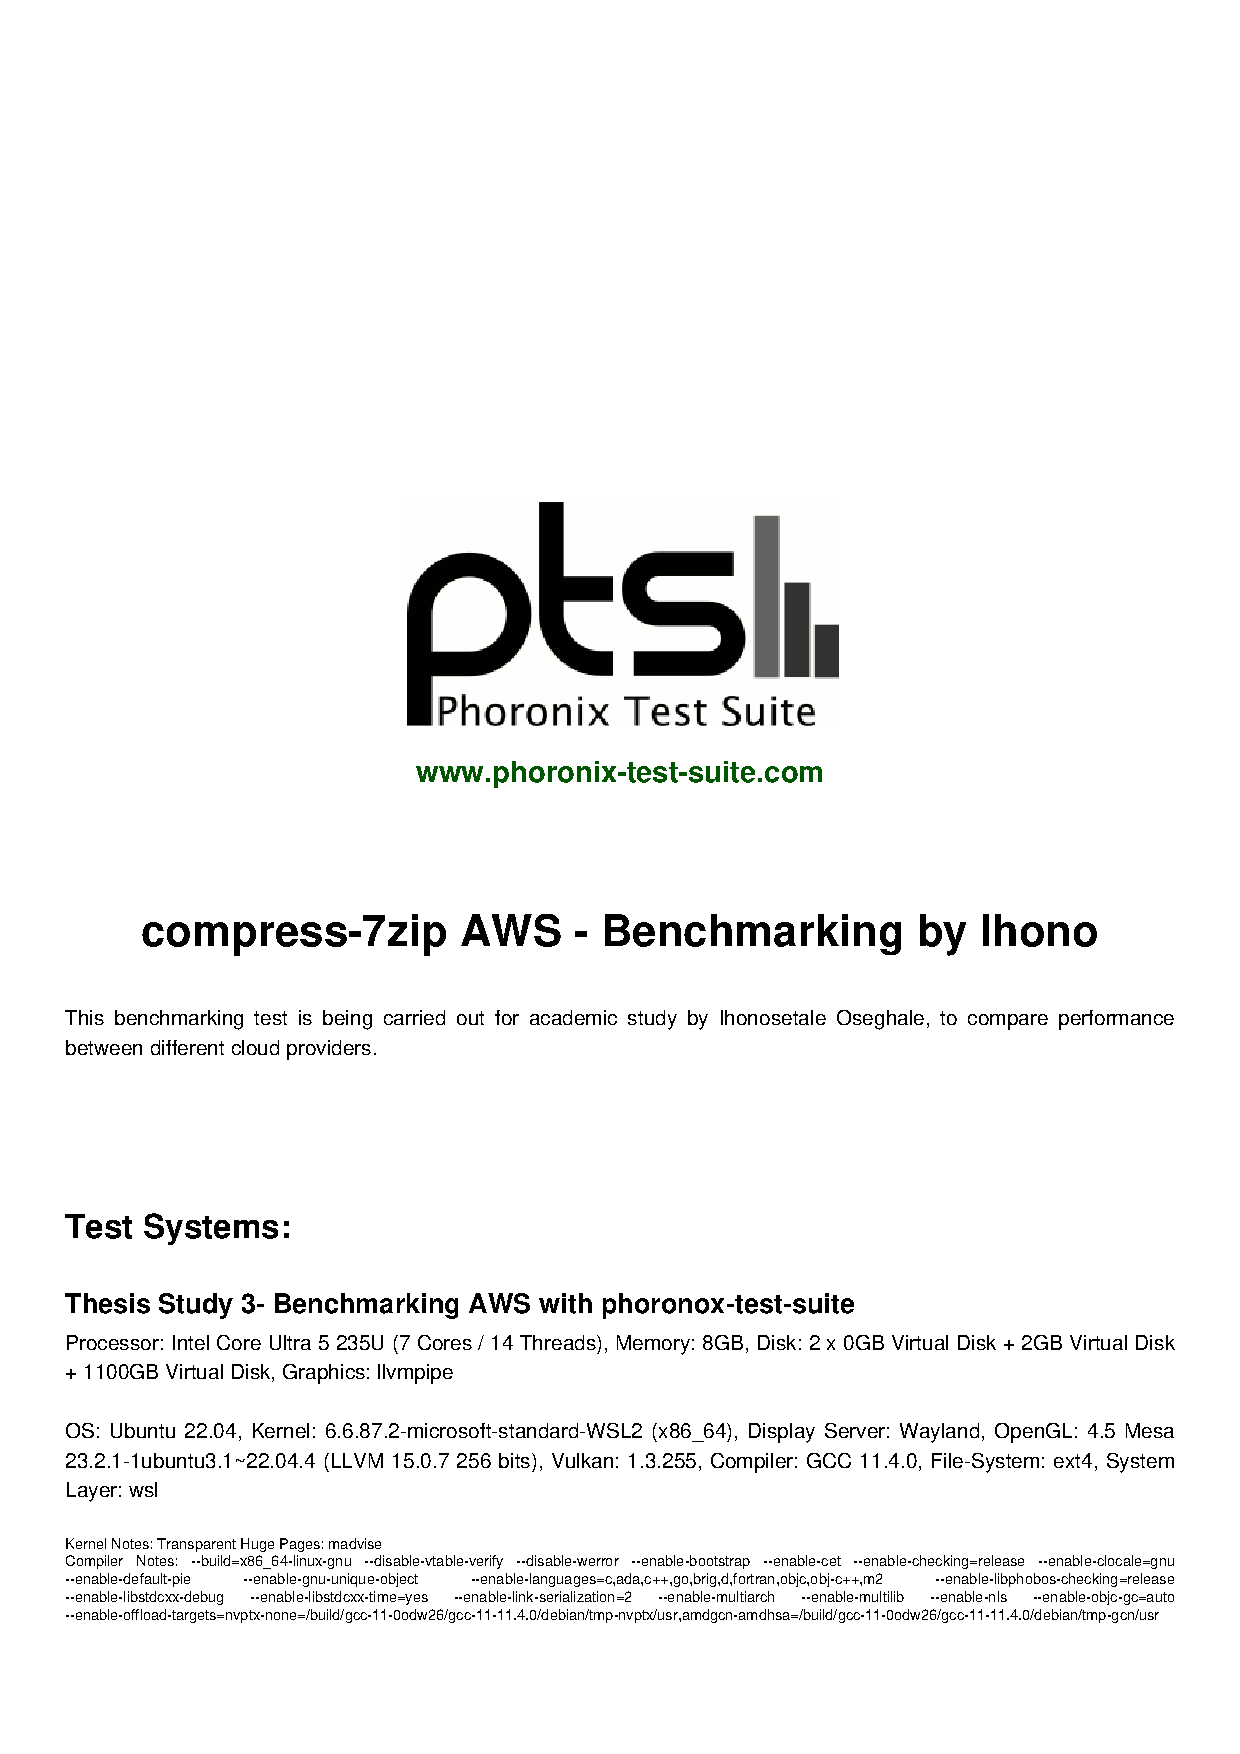
\includegraphics[page=1, width=0.47\textwidth]{phoronix-7zip-trial-report.pdf}}\hfill
  \fbox{\includegraphics[page=3, width=0.47\textwidth]{phoronix-7zip-trial-report.pdf}}
  \caption{A Phoronix Test Suite report from a trial run of the 7-Zip test on a local
           laptop. Not used for any result in this thesis.}
  \label{fig:pts-trial-report}
\end{figure}
